\documentclass{beamer}
\usepackage[utf8]{inputenc}

\usepackage{multirow}


\usetheme{Madrid}
\usecolortheme{default}

\title[Python navigation] %optional
{Python Modules for Marine Navigation}
\subtitle{An alternative to GNSS}

\author[Cédric MARCHAND] % (optional)
{Cédric Marchand}

\institute[Lab-STICC] % (optional)
{
  Lab-STICC, Université de Bretagne Sud
}

\date[\today] {\today}

% Multiple logos
\titlegraphic{
        
    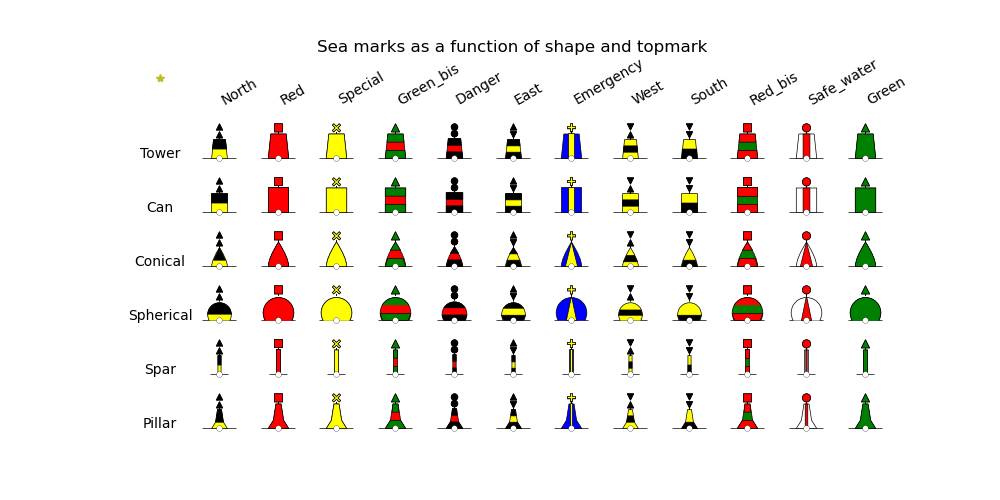
\includegraphics[width=5cm]{./pictures/marker1.png}
    \hspace{1cm}
    \includegraphics[width=5cm]{./pictures/waypoints.png}
    \hspace{1cm}
    
\includegraphics[width=1cm]{./pictures/logo-cnrs.png}
    \hspace{1cm}
    
\includegraphics[width=2cm]{./pictures/logo-ubs.png}
    \hspace{1cm}
    
\includegraphics[width=2cm]{./pictures/logo-lab-sticc.png} 
}

\logo{
\includegraphics[width=1cm]{./pictures/logo-lab-sticc.png}}

\AtBeginSection[]
{
  \begin{frame}
    \frametitle{Table of Contents}
    \tableofcontents[currentsection]
  \end{frame}
}

\begin{document}


\frame{\titlepage}


\begin{frame}
\frametitle{Table of Contents}
\tableofcontents
\end{frame}



\section{Introduction}

\begin{frame}
\frametitle{Introduction: Alternative to GNSS}
    \begin{columns}
    \column{0.5\textwidth}
        What are the alternatives to the Global Navigation Satellite Systems (GNSS)
    \column{0.5\textwidth}
        \begin{figure}[h]
        \centering
        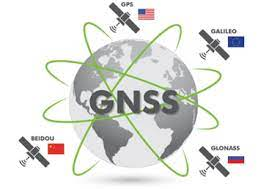
\includegraphics[height=3cm]{./pictures/GNSS.jpeg}
        \end{figure}
    \end{columns}
    
    \begin{itemize}
        \item Celestial navigation
        \item \textbf{Visual-aided navigation}
        \item Navigation by signal of opportunity (radio, WiFi ...)
        \item Magnetic navigation
        \item Bathymetric navigation
        \item Inertial navigation (dead reckoning)
        \item ...
        \item Fusion of previously cited techniques
    \end{itemize}
\end{frame}


\begin{frame}
\frametitle{Introduction: Python module}
    
        \begin{columns}
    \column{0.5\textwidth}
        Why Python?
        \begin{itemize}
            \item Python is used in many projects ( machine learning, image recognition)
            \item lots of libraries (NumPy, Matplotlib, Cartopy, ...)
            \item No navigation tools (to my knowledge) available in Python
        \end{itemize}
    
    \column{0.5\textwidth}
        New modules
        \begin{itemize}
            \item to extend the set of markers used in Matplotlib with the nautical symbol
            \item Navigation tools
        \end{itemize}
    \end{columns}

        \begin{figure}[h]
        \centering
        
\includegraphics[height=1.5cm]{./pictures/python.jpeg}
        
\includegraphics[height=1.5cm]{./pictures/numpy.png}
        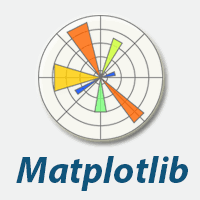
\includegraphics[height=1.5cm]{./pictures/matplotlib.png}
        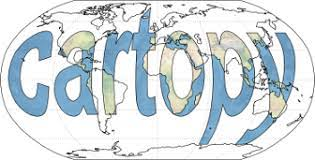
\includegraphics[height=1.5cm]{./pictures/cartopy.jpeg}
        \end{figure}


\end{frame}

\section{Nautical Marks for Pyplot markers }
\begin{frame}
    \begin{figure}[l]
    \centering
    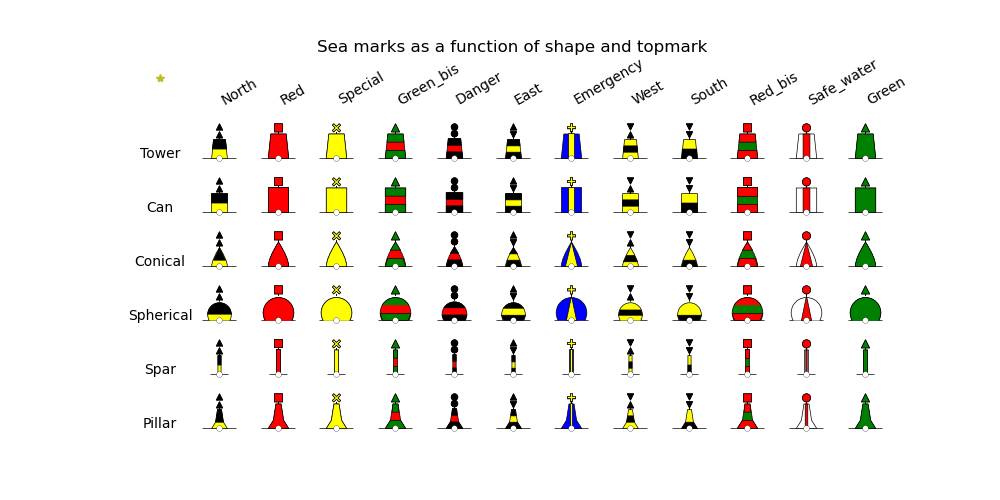
\includegraphics[width=12cm]{./pictures/marker1.png}
    \caption{Sea marks for Matplotlib marker  }
    \end{figure}
\end{frame}


\begin{frame}
    \begin{figure}[h]
    \centering
    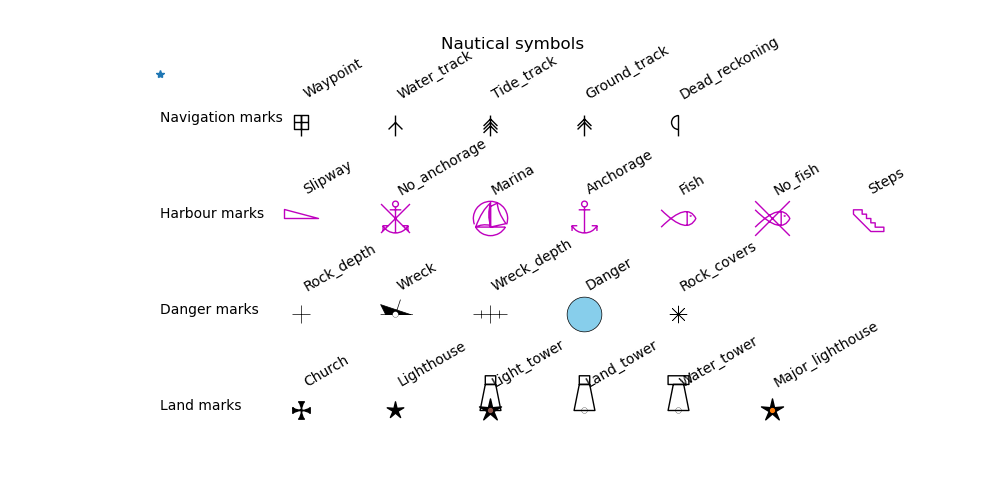
\includegraphics[width=12cm]{./pictures/marker2.png}
    \caption{Nautical symbols for Matplotlib marker  }
    \end{figure}

\end{frame}


\begin{frame}
    \frametitle{Marker on a map [1]}
    \begin{figure}[h]
    \centering
    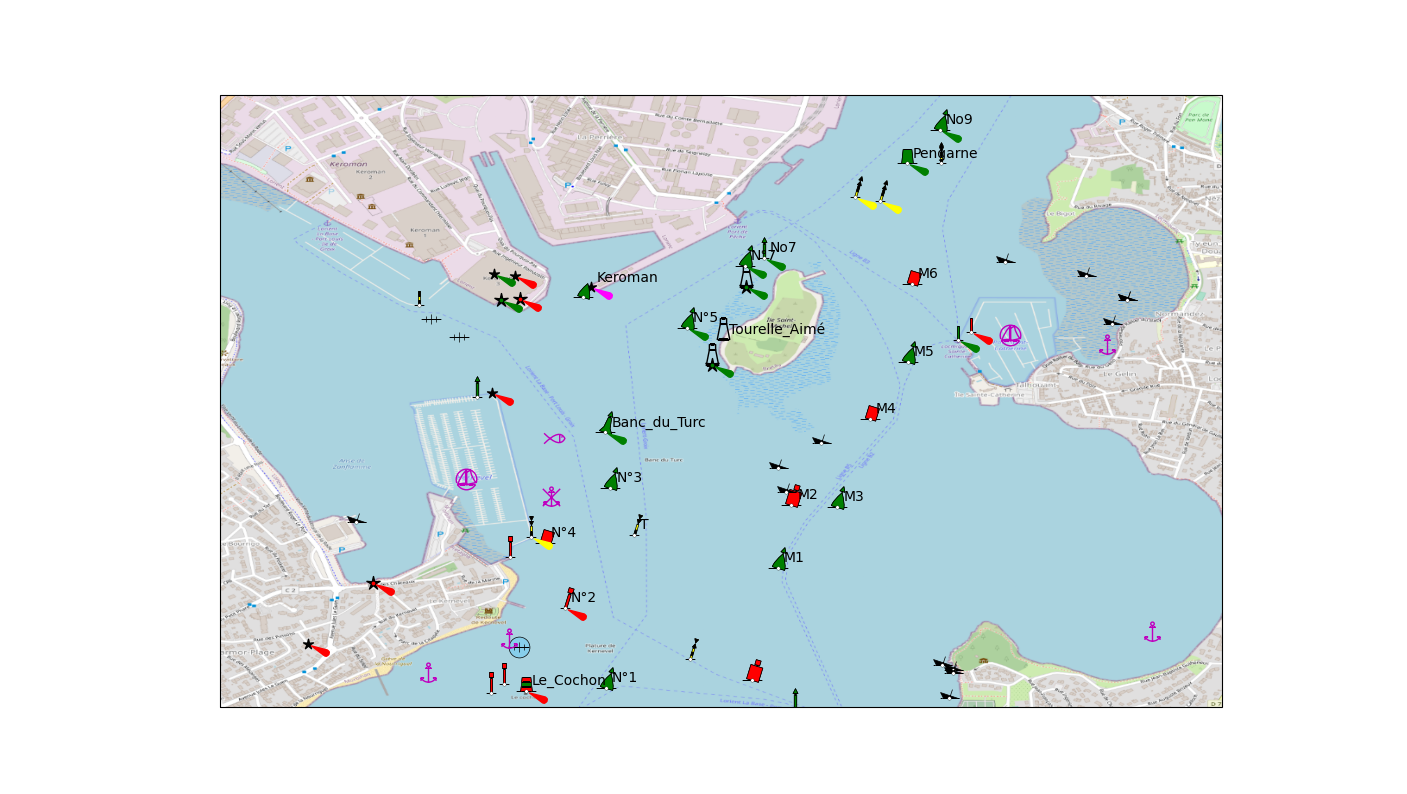
\includegraphics[width=12cm]{./pictures/map_marker.png}
    \end{figure}
    %{ \tiny Markers are added using a CSV file:
    %"-3.36396, 47.72219, pillar, green, green, Banc du Turc, True" produces a floating green pillar named "Banc du turc" with green light %at position -3.36396E, 47.72219N}
    [1] \href{https://www.openseamap.org/}{openseamap} 
\end{frame}

\section{Line of Position (LOP) Fix}

\begin{frame}
    \frametitle{Traditional "cocked hat" 3LOP Fix}
    \begin{figure}[h]
    \centering
    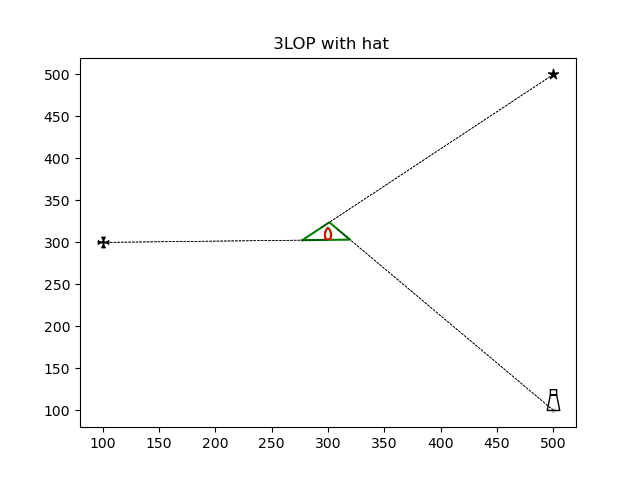
\includegraphics[width=10cm]{./pictures/3LOP_hat.png}
    \end{figure}
\end{frame}


\begin{frame}
    \frametitle{3LOP Fix with error bars [1]}
    \begin{figure}[h]
    \centering
    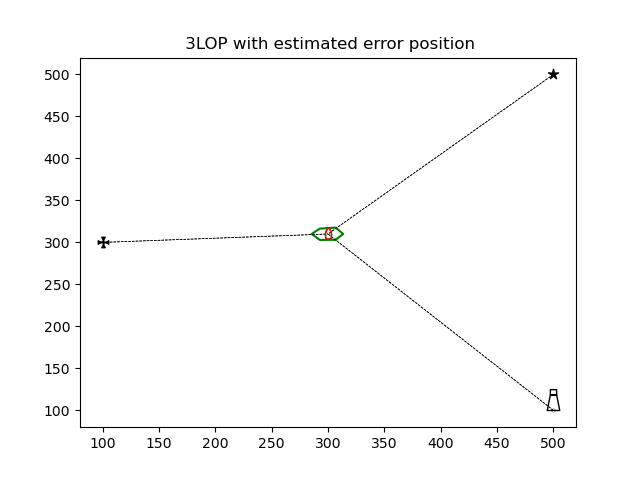
\includegraphics[width=10cm]{./pictures/3LOP_estim.png}
    \end{figure}

[1] \href{https://www.starpath.com/resources2/Bearing_Fix_Accuracy.pdf}{David brush, "Notes on Bearing Accuracy"}

\end{frame}


\begin{frame}
    \frametitle{3LOP Fix: "Cocked Hat" Versus "Error bars" fix}
    \begin{columns}
    \column{0.5\textwidth}
        \begin{figure}[h]
        \caption{Traditional cocked hat}
        \centering
        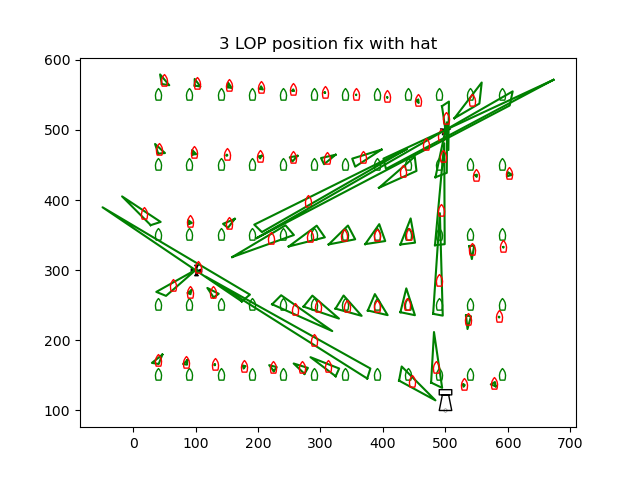
\includegraphics[height=4.5cm]{./pictures/3LOP_hat2.png}
        \end{figure}
    
    \column{0.5\textwidth}
        \begin{figure}[h]
        \caption{Error bar }
        \centering
        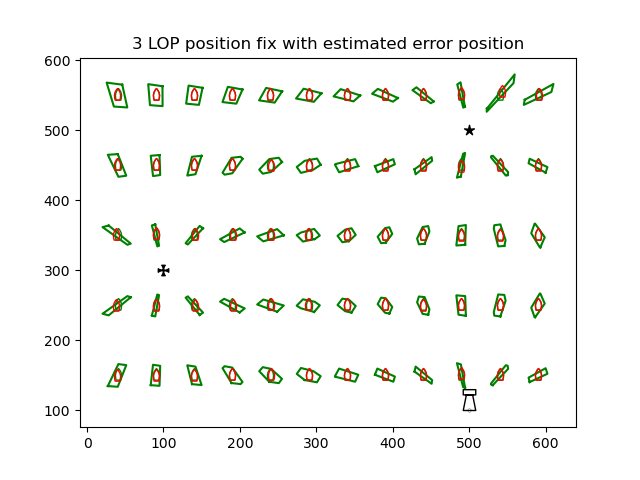
\includegraphics[height=4.5cm]{./pictures/3LOP_estim2.png}
        \end{figure}
    \end{columns}
\end{frame}


\begin{frame}
    \frametitle{Select best 3LOP}
    \begin{figure}[h]
    \centering
    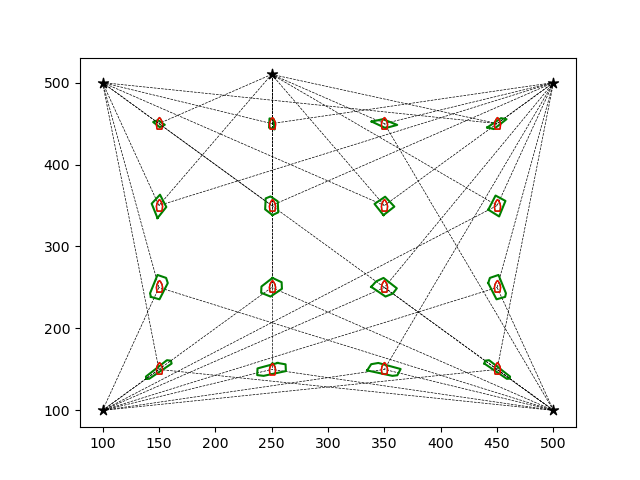
\includegraphics[width=10cm]{./pictures/select_3LOP.png}
    \end{figure}
\end{frame}

\section{Running fix}

\begin{frame}
    \frametitle{Running Fix}
    \begin{figure}[h]
    \centering
    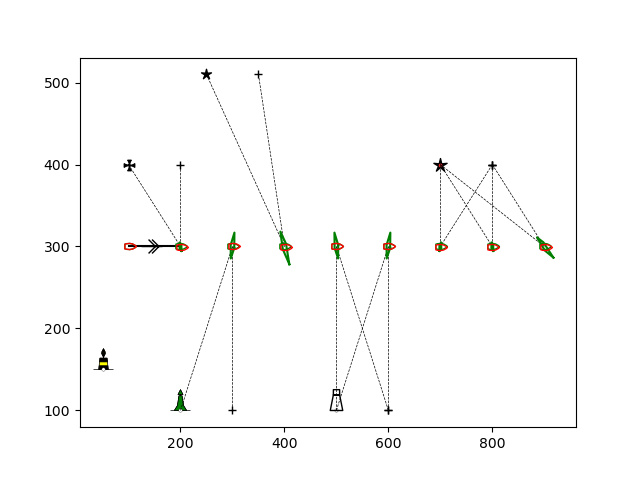
\includegraphics[width=10cm]{./pictures/runing_fix.png}
    \end{figure}
    Running fix with select of mark closest to a 90-degree angle
\end{frame}

\section{Course of steer}

\begin{frame}
    \frametitle{Course of steer}

    A course to steer is a method of calculating what heading the boat needs to be pointing at in order to get successfully to its way-point considering the effects of tide and leeway. 
    \begin{columns}
    \column{0.5\textwidth}

        \begin{itemize}
            \item $ >>> $ Tide vector
            \item $ >> $ Ground vector
            \item $ > $ Water vector
        \end{itemize}
    
    \column{0.5\textwidth}
        \begin{figure}[h]
        \centering
        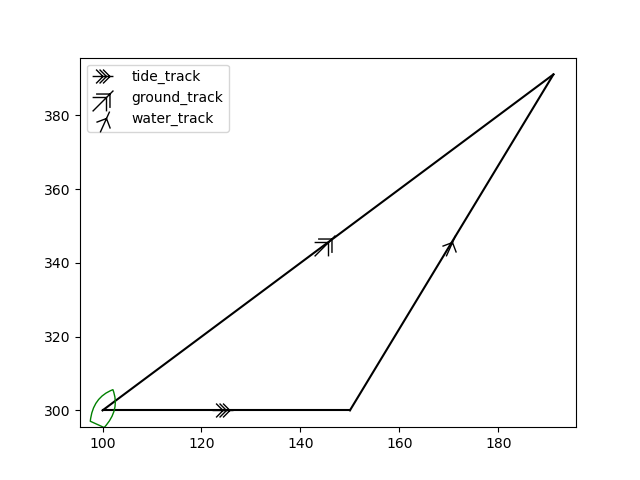
\includegraphics[height=4.5cm]{./pictures/course_of_steer.png}
        \end{figure}
    
    \end{columns}
\end{frame}

\section{Waypoints}

\begin{frame}
    \frametitle{Waypoints}

        \begin{figure}[h]
        \centering
        \includegraphics[width=12cm]{waypoints.png}
        \end{figure}
        
\end{frame}
    


\section{Conclusion}

\begin{frame}
\frametitle{Conclusion}
Python modules for 
    \begin{itemize}
        \item Nautical marks
        \begin{itemize}
            \item Sea marks
            \item Symbol marks
        \end{itemize}
        \item Backend marine navigation
        \begin{itemize}
            \item 3LOP fix
            \item Running Fix
            \item Course of steer
            \item Waypoints
        \end{itemize}
        \item Python modules available on GitHub
        \begin{itemize}
            \item https://github.com/cedricomarchando/navigation
        \end{itemize}
        
    \end{itemize}
\end{frame}

\section{Future work}

\begin{frame}
    \frametitle{Future work}
    \begin{itemize}
        \item More nautical marks, add light period, improve graphic quality
        \item More maps, wrapper to use existing maps
        \item Unit choice and conversion (mph, knots, miles, km, ms ...)
        \item Wrapper to add existing mark positions, coastline, depth
        \item Nautical navigation front end (bearing, mark detection, etc.)
        \item Improve position estimate
        \item Promotion, valorization, publication, license
        \item Add collision avoidance
        \item Fusion with IMU
        \item Comparison with state-of-the-art
        \item Back end for celestial navigation
        \item ...
    \end{itemize}s
\end{frame}



\end{document}

